\documentclass[tikz,border=3.14mm]{standalone}
\usepackage{tikz}
\usepackage[dvipsnames]{xcolor}

\begin{document}
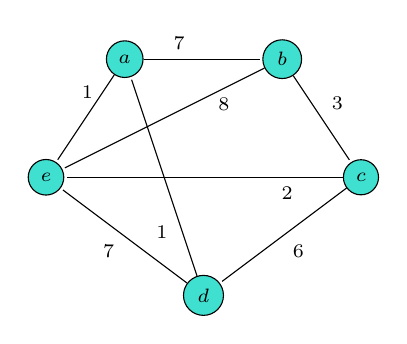
\begin{tikzpicture}[shorten >=1pt, node distance=2cm, auto, scale=1]
    \tikzstyle{vertex}=[draw, fill=Turquoise, circle, inner sep=0.1cm, font=\scriptsize]
    \tikzstyle{edge}=[font=\scriptsize]
    
    % Vertices at custom coordinates with labels in math mode and turquoise color
    \node[vertex] (a) at (-1, 1.5) {$a$};
    \node[vertex] (b) at (1, 1.5) {$b$};
    \node[vertex] (c) at (2, 0) {$c$};
    \node[vertex] (d) at (0, -1.5) {$d$};
    \node[vertex] (e) at (-2, 0) {$e$};
    
    % Edges with weights
    \path[draw]
      (a) edge[pos=0.2, left] node[edge] {1} (e)
      (a) edge[pos=0.3] node[edge] {7} (b)
      (b) edge node[edge] {3} (c)
      (c) edge node[edge] {6} (d)
      (d) edge node[edge] {7} (e)
      (d) edge[pos=0.3] node[edge] {1} (a)
      (c) edge[pos=0.2] node[edge] {2} (e)
      (b) edge[pos=0.2, below] node[edge] {8} (e);
\end{tikzpicture}

\end{document}
